% THIS IS SIGPROC-SP.TEX - VERSION 3.1
% WORKS WITH V3.2SP OF ACM_PROC_ARTICLE-SP.CLS
% APRIL 2009
%
% It is an example file showing how to use the 'acm_proc_article-sp.cls' V3.2SP
% LaTeX2e document class file for Conference Proceedings submissions.
% ----------------------------------------------------------------------------------------------------------------
% This .tex file (and associated .cls V3.2SP) *DOES NOT* produce:
%       1) The Permission Statement
%       2) The Conference (location) Info information
%       3) The Copyright Line with ACM data
%       4) Page numbering
% ---------------------------------------------------------------------------------------------------------------
% It is an example which *does* use the .bib file (from which the .bbl file
% is produced).
% REMEMBER HOWEVER: After having produced the .bbl file,
% and prior to final submission,
% you need to 'insert'  your .bbl file into your source .tex file so as to provide
% ONE 'self-contained' source file.
%
% Questions regarding SIGS should be sent to
% Adrienne Griscti ---> griscti@acm.org
%
% Questions/suggestions regarding the guidelines, .tex and .cls files, etc. to
% Gerald Murray ---> murray@hq.acm.org
%
% For tracking purposes - this is V3.1SP - APRIL 2009

\documentclass{acm_proc_article-sp}
\usepackage{graphicx}
\usepackage{listings}
\usepackage{subcaption}
\usepackage[justification=centering]{caption}
\graphicspath{{images/}}

%\lstset{%frame=tb,
%  language=C,
%  %aboveskip=3mm,
%  %belowskip=3mm,
%  showstringspaces=false,
%  columns=flexible,
%  basicstyle={\small\ttfamily},
%  %numbers=none,
%  %numberstyle=\tiny\color{gray},
%  %keywordstyle=\color{blue},
%  %commentstyle=\color{dkgreen},
%  %stringstyle=\color{mauve},
%  breaklines=true,
%  breakatwhitespace=true,
%  tabsize=4
%}

\begin{document}

\title{Efficient Data Retrieval from a Secure, Durable, Append-Only Log
\titlenote{This paper was written at the University of California at Berkeley as a CS 262A class project. For more info see \texttt{http://www.cs.berkeley.edu/~kubitron/courses/cs262a-S16/index\_projects.html}}}
%
% You need the command \numberofauthors to handle the 'placement
% and alignment' of the authors beneath the title.
%
% For aesthetic reasons, we recommend 'three authors at a time'
% i.e. three 'name/affiliation blocks' be placed beneath the title.
%
% NOTE: You are NOT restricted in how many 'rows' of
% "name/affiliations" may appear. We just ask that you restrict
% the number of 'columns' to three.
%
% Because of the available 'opening page real-estate'
% we ask you to refrain from putting more than six authors
% (two rows with three columns) beneath the article title.
% More than six makes the first-page appear very cluttered indeed.
%
% Use the \alignauthor commands to handle the names
% and affiliations for an 'aesthetic maximum' of six authors.
% Add names, affiliations, addresses for
% the seventh etc. author(s) as the argument for the
% \additionalauthors command.
% These 'additional authors' will be output/set for you
% without further effort on your part as the last section in
% the body of your article BEFORE References or any Appendices.

\numberofauthors{4} %  in this sample file, there are a *total*
% of EIGHT authors. SIX appear on the 'first-page' (for formatting
% reasons) and the remaining two appear in the \additionalauthors section.
%


\author{
\begin{tabular}{cc}
Sam Kumar,
Andrew M. Chen,
Paul R. Bramsen,
John D. Kubiatowicz\\
\{samkumar, andrewmchen, paulbramsen, kubitron\}@berkeley.edu\\ \\
Electrical Engineering and Computer Sciences, UC Berkeley\\
\end{tabular}
}
% There's nothing stopping you putting the seventh, eighth, etc.
% author on the opening page (as the 'third row') but we ask,
% for aesthetic reasons that you place these 'additional authors'
% in the \additional authors block, viz.
%\additionalauthors{Additional authors: John Smith (The Th{\o}rv{\"a}ld Group,
%email: {\texttt{jsmith@affiliation.org}}) and Julius P.~Kumquat
%(The Kumquat Consortium, email: {\texttt{jpkumquat@consortium.net}}).}
\date{10 May 2016}
% Just remember to make sure that the TOTAL number of authors
% is the number that will appear on the first page PLUS the
% number that will appear in the \additionalauthors section.

\maketitle
%\begin{abstract}
%The Global Data Plane (GDP) \cite{GDP} provides a secure, verifiable, append-only, single-writer log interface where logs are replicated across a range of possibly untrusted hosts. A major advantage of such a log interface is that it is possible to provide atomicity and consistent replication with little overhead (where a log entry is the basic atomic unit). In this paper, we present the Global Data Plane File System (GDPFS), a traditional filesystem built on top of the GDP log absitraction. Our motivation to do this is twofold. First, we would like to open the atomicity and security properties of the GDP to a wider variety of use cases. Second, we would like to evaluate the effectiveness of the GDP as a primitive for building complex distributed systems, based on both the performance of the resulting filesystem and our experience in creating it.
%\end{abstract}

\begin{abstract}
The Global Data Plane (GDP) \cite{GDP} provides a secure, verifiable, append-only, single-writer log interface where logs are replicated across a range of possibly untrusted hosts. A major advantage of such a log interface is that it is possible to provide atomicity and consistent replication with little overhead, while scaling at a global level. However, expressing mutable objects in append-only logs, while simultaneously providing efficient access to data within those objects, is a nontrivial task. In this paper, we present the Global Data Plane File System (GDPFS), a distributed filesystem that expresses mutable files within append-only logs and provides efficient data access within files. Because it is built on top of the GDP, the GDPFS has the potential to scale very well and run securely on untrusted hardware.
\end{abstract}

% A category with the (minimum) three required fields
%\category{H.4}{Information Systems Applications}{Miscellaneous}
%A category including the fourth, optional field follows...
%\category{D.2.8}{Software Engineering}{Metrics}[complexity measures, performance measures]

%\terms{Algorithms, Design, Performance, Reliability, Security}

%\keywords{Filesystem, Global Data Plane, Log, FIG Tree} % NOT required for Proceedings

\section{Introduction}
The Global Data Plane (GDP) \cite{GDP} provides a substrate for storing data that can run securely on untrusted hardware. The basic primitive that it exports to applications is a verifiable, append-only, single-writer log. With such a log interface, it is possible to provide atomicity and consistent replication with little overhead (where a log entry is the basic atomic unit). Traditionally, systems that aim to provide rich data semantics first build the functionality that they need, and then layer schemes to enforce such data semantics on top of the functionality. Database Management Systems are a good example of this. First the system implements its main functionality, namely allowing the creation of relations and the retrieval of data from them. Then, to achieve the desired data semantics, it may employ schemes such as Write-Ahead Logging \cite{ARIES}, Two-Phase Locking \cite{CCRDBS}, Key-Range Locking \cite{KRLSIC}, etc. on top of the existing functionality in the system.

In contrast, the GDP provides a primitive, namely a single-writer log, for which these desirable properties can be supported more easily than in a database. Because the logs are \emph{append-only}, replicas can be kept consistent without a write-ahead logging scheme. Furthermore, it is easy to verify authenticity of the logs because each entry will have a fixed signature at write time.

As data-collecting sensors become pervasive, the GDP is obviously much more well-suited to storing their data than a traditional DBMS, for the simple reason that a DBMS must support much richer data semantics than are needed for this task. Beyond being more efficient, the GDP enables a new paradigm for building complex distributed data systems; rather than first building the system and then adding locking or logging schemes to achieve the desired consistency and durability properties, one may choose to build a system on top of GDP, which can cheaply achieve these properties, in such a way that some of these properties shine through in the final system.

The main difficulty in this approach is one of the advantages mentioned earlier: the append-only nature of logs in the Global Data Plane. In addition to being well-suited for use cases in which data is only added, and never removed, the GDP is aimed more generally at providing secure data transport for cloud services. One natural way the GDP could be used to this end is as support for a log-based messaging scheme. Apache Kafka \cite{Kafka}, for example, is a publish-and-subscribe messaging service based on a log. However, it is also desirable to provide richer semantics such as data mutability on top of the GDP. In particular, we wish to provide the abstraction of a shared file that can be written by its owner, and read by other entities\footnote{The single-writer restriction stems from the fact that the GDP provides a \emph{single-writer} log as its main abstraction.}. The append-only nature of logs in the GDP makes this a nontrivial task; while adding new data to a file is easy, our goal is to record \emph{mutations} to data in an append-only log while simultaneously providing a means to efficiently retrieve that data.

In this paper, we present the Global Data Plane File System (GDPFS), a traditional distributed filesystem built on top of the GDP log abstraction. Our motivation to do this is twofold. First, we would like to open the atomicity and security properties of the GDP to a wider variety of use cases. Second, we would like to evaluate the effectiveness of the GDP as a primitive for building complex distributed systems, based on both the performance of the resulting filesystem and our experience in creating it.

\section{Overview of the GDPFS}
\begin{figure}[t]
\centering
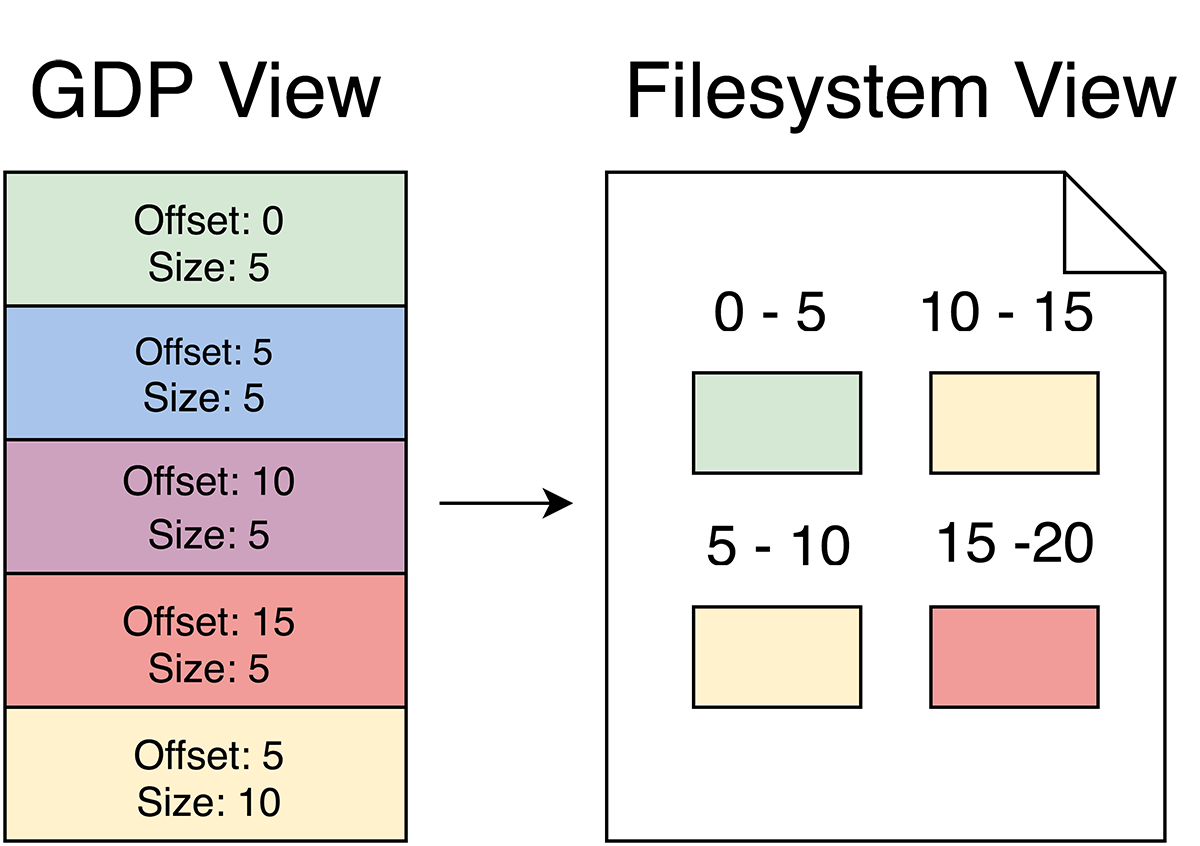
\includegraphics[width=.6\columnwidth]{gdpfs_basic_file}
\caption{Basic layout of a GDPFS file\label{fig:gdpfs_basic_file}}
\end{figure}
As with most filesystems, the basic unit of storage in the GDPFS is a file. All other filesystems constructs---such as directories, symbolic links, etc.---can be built on top of basic files. Thus building a basic file which could be efficiently read from and written to in a way that guaranteed desired ACID semantics was our primary focus when building the GDPFS. The design we settled upon is described in this section. The implementation details of this design are described in Section \ref{sec:implementation}.

Each file in the GDPFS is backed by a single log in the GDP. Files are modified by appending entries to the log specifying a range of bytes and the new bytes that that range is to take on. This means that new writes can eclipse old writes simply by specifying an overlapping offset and size. Since the GDP accepts appends to logs atomically, all writes to files are guaranteed to be atomic.

Reads are satisfied by scanning the log backwards and retaining bytes that fall within the range of bytes being read as they are seen. Note that it is essential that the log be scanned backwards. The same logical byte may have been written multiple times but we are interested in the most recent version. See Figure \ref{fig:gdpfs_basic_file} for a depiction of how this works.

While the previously described system is correct, it is not efficient. Writes can be done in time constant in the number of log entries and logical file size. Unfortunately, it may be necessary for a read to examine every log entry (for example when the read needs data that is in the first log entry) so reads can take time proportional to the length of the log. In order to solve this issue, we implemented a number of caching and indexing strategies.

As a first step toward performance, we cache reads and writes on the local filesystem. This gives us gains on reads, in two ways. First and most importantly, if we have a cache hit we can avoid going to the GDP at all, which completely eliminates the need to hit the network even once. This advantage is magnified if multiple network accesses would have been necessary in order to locate and retrieve relevant blocks. Second, we no longer spend CPU time reconstructing blocks based on log entries. We use a write-through asynchronous policy, allowing readers to be kept up-to-date without incurring the network latency on the writes. See Section \ref{sec:implementation_file_cache} for additional details.

If the bytes of interest are not in the cache, then clearly we have to hit the GDP to retrieve the necessary data. This once again brings up the problem of reads taking time linear in the size of the log, which is not acceptable performance. We solve this through use of a special tree index structure called a FIG Tree, described in detail in section \ref{sec:implementation_fig_tree}. A FIG tree allows bytes to be found in time \emph{logarithmic} in the size of the \emph{file}, much better than \emph{linear} in the size of the \emph{log}. The FIG tree is updated on writes and periodically\footnote{Due to time constraints, our current implementation does not checkpoint files periodically; rather it writes the checkpoint entry when the in-memory representation of the file is discarded.} pushed to the GDP in a special checkpoint log entry. Updating the FIG tree adds a small cost to writes, no worse than logarithmic in the size of the file. Since we expect frequent access of FIG tree indexes for files in active use, we keep an in-memory partial representation, pulling in subtrees as they are accessed. Furthermore we cache the checkpoint log entries as they are read in since it is likely that related subtrees will live in the same checkpoints. Figure \ref{fig:gdpfs_overview} illustrates how the system fits together.

\begin{figure}[t]
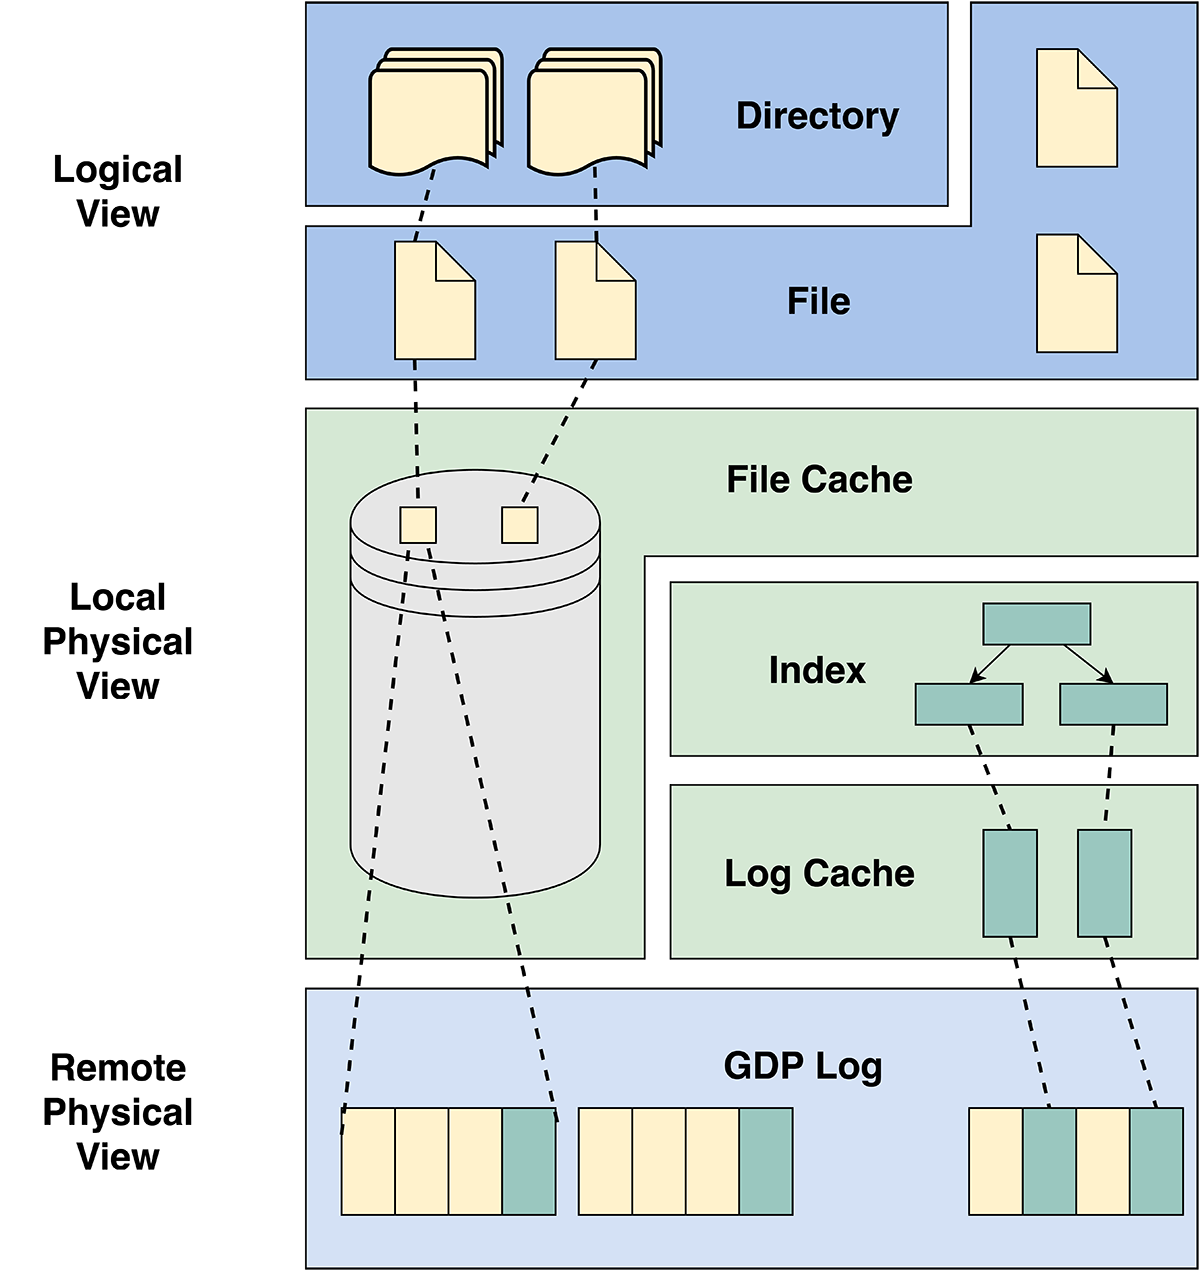
\includegraphics[width=\columnwidth]{gdpfs_overview}
\caption{Overview of the GDPFS structure. Data flows between vertical boundaries.\label{fig:gdpfs_overview}}
\end{figure} 

\section{Implementation}\label{sec:implementation}

Since we only had about 2 months to build a working performant prototype of the GDPFS, we had to carefully choose tools to would speed development while incurring minimal performance overhead (e.g. FUSE). This section describes the process we went through in selecting these tools and gives an in-depth explanation of the techniques we used to achieve our performance goals.

\subsection{FUSE}   
The implementation of the GDPFS is entirely built upon the Filesystem in Userspace library (FUSE) \cite{FUSE}. This library enables programmers to implement entire filesystems in userspace and works by redirecting all syscalls issued to a FUSE mounted filesystem to a special user level process. 

For example, when a user tries to open a file, the FUSE library in kernel space will forward this syscall to the handler running in our user level process. In this handler for open we first enforce the permissions on this file and then tell FUSE to make all subsequent requests to this specific file with a file handle that we specify. Finally, FUSE will return the results of a successful open with a process specific file descriptor that is different than the file handle that we have specified. Later, when that same process makes another syscall with this file descriptor, the FUSE library will recognize this (PID, FD) pair and call the correct user level handler with the appropriate file handle which we specified on the open. Upon returning from this user level handler, the results of that syscall will be shuffled back into the kernel and then finally to the process which issued that syscall.

We chose to build our filesystem on top of FUSE ultimately because it allowed us to avoid writing any kernel level code. This way it was much easier rapidly iterate on our filesystem without worries of a bad line of code bricking our computer. However, building a filesystem this way is not without its limitations. For example, in FUSE each filesystem syscall incurs an additional pair of user space to kernel space transitions. This makes FUSE inherently slower than filesystems built in the kernel. Also, because our FUSE-based implementation is running in userspace, it is impossible to directly access the block-store. Instead, any sort of disk accesses we make must go through a separate filesystem. Although our current prototype of the GDPFS is built using FUSE due to its ease of use, a more stable and permanent version would foreseeably be written directly in the kernel.


\subsection{File Caching Layer}\label{sec:implementation_file_cache}
Reads to files in the GDPFS first check a cache stored on the local disk. The underlying implementation of this cache is a file on the local filesystem which mirrors the logical view of the file on the GDPFS.

The way the cache works is very simple. Each read first checks to see if it can be satisfied by the file cache. If this is not possible then we must go to the remote log to find out the contents of this range. Upon reading from the remote log we would populate the appropriate parts of the file cache. On writes, we simply populate the appropriate portion of the cache and issue an asynchronous write to the GDP before returning. Because of this, all writes can return without waiting for any network I/Os\footnote{The correctness of this scheme depends on asynchronous requests being processed in the same order that they are made. For the current implementation of the GDP we believe this to be the case. If this changes, we could create a bounded buffer of requests, and a worker thread that processes them synchronously. Rather than making a request to the log daemon asynchronously, we would just enqueue the request into the buffer, achieving the desired semantics.}.

An alternative caching scheme that we could have used to locally store data in files is to treat the local disk as a general cache for log entries read from the GDP. However, we believe that materializing files directly, as described above, is strictly better for two reasons. First, storing the log entries directly would also store stale data (i.e., data that has since been overwritten), wasting space in the local disk. Second, it let us use the local filesystem (ext4), which is well-optimized for performance, to store parts of the same file close to each other on disk.

\subsubsection{Sparse Caching}
Because we only cache portions of a file that have been accessed, the cached version of a file may be incomplete and have portions which are not valid.

Originally, each per-file cache was implemented through two files on the local filesystem. One file would be responsible for storing the actual contents of the file whereas the other would be a bitmap which could be used to tell which bytes in the cache were actually valid. The $n$th bit of the bitmap and the $n$th byte of the locally cached file correspond to the $n$th byte in the logical view of the file. Thus, reads to the cache would first check the bitmap to make sure the cache was valid and then would read that range of bytes in the mirrored cache file. Because it is possible to write past the end of the file in ext4 without actually allocating the blocks for the empty regions, this method was an acceptable way for us to create partially cached copies of GDPFS files without paying the space for the entire file.

However, having a bitmap for every file adds a significant amount overhead to the space of our cache. Specifically, for every $n$ cached bytes, we pay an additional $\left\lceil\frac{n}{8}\right\rceil$ bytes to keep track of the bitmap. To avoid this overhead, we attempted to use a feature of modern filesystems intended for use on sparse files. In addition to not allocating blocks for holes created by writing past the end of the file, ext4 also keeps track of the positions of these holes internally. For example, using the SEEK\_HOLE option with lseek will move the file offset to the next hole greater than or equal to the argument offset. Because of this functionality, finding out if a range $[a,b)$ in our cache is valid should theoretically be reduced to checking if the result of lseek(a, SEEK\_HOLE) is greater than or equal to b. However, the granularity to which ext4 tracks these holes is at the blocksize level so holes inside a partially filled in block will not be reported using lseek(SEEK\_HOLE). 

Throughout our testing, we have not yet run into any issues with this bug since it is unusual for a process to write a part of a block on a cold cache and then read a different part of this block later. Because of time limitations, we have decided to revert to keeping a bitmap for each file because our performance is not bound by checking ranges on the bitmap. 

For future work, it may be desirable to combine the bitmap and the SEEK\_HOLE functionality in order to proverbially get the best of both worlds. For example, one simple way to use both is to first check using SEEK\_HOLE if the block we are reading is valid. If it is not, then we can entirely avoid having to check that portion of the bitmap. Otherwise, we must still check the bitmap since there may be portions of this block that are invalid.

\subsubsection{File Cache Coherency}
One other aspect that we considered is the consistency of our file cache. Because we the single-writer semantics of the underlying GDP through to the GDPFS, we avoided dealing with a majority of adversarial cases that would leave our cache inconsistent. However, it is possible that a single private key could be used on two separate hosts. In this case, although there is one entity in the security sense of the word, we must maintain a pair of consistent caches across two separate hosts. One idea that we are considering for future work is to create a service that provides the filesystem to multiple users, and serializes the writes to the logs as a single writer (because the GDP logs are \emph{single-writer}). Many of the same consistency issues we would see in such a setting also arise in the case of a single writer mounting the same GDPFS in multiple places and interacting with the separate mounts concurrently. Therefore, we provide in this section a discussion of some of the difficulties that arise in such a case.

Suppose Alice and Bob both open a file, as writers, on the GDPFS. Consider, as a simple case, the scenario where Alice and Bob concurrently write different values to the same range of byte in the file. To make the example concrete, consider the case where Alice writes byte sequence $A$ to the first 100 bytes of the file, and Bob writes the byte sequence $B$ to the first 100 bytes of the file. The standard way in which the GDP allows one entity to be informed of new writes to a log is via a \emph{subscription} to the log. In the example, Alice first writes $A$ to her cache, and Bob first writes $B$ to his cache; meanwhile, they both asynchronously make requests to the GDP log server. The log server will then choose some serial ordering for these writes and append both entries to the log; then, Alice and Bob will be informed of each other's writes via the subscription. Alice will write $B$ to her cache, and Bob will write $A$ to his cache. After this is finished, Alice will think that the first 100 bytes of the file contain $B$, whereas Bob will think that the first 100 bytes of the file contain $A$. In particular, either Alice's cache or Bob's cache will be incorrect until he or she remounts his or her filesystem.

One way to achieve consistency is to treat the order in which updates are sent due to the subscription to a file as describing the ground-truth ordering of writes to the file. After making an asynchronous request to append to a log, a client receives first an application-layer ACK from the log server, and then the same log entry in response to the client's subscription to the log. Upon receipt of the ACK, Alice would check its record number to see if it is what she would expect if she were the only writer; if it is what she expects, then she can be sure that no writes happened in between. If the record number is higher than expected, then Alice can conclude that a separate writer made a write to the file before her write. Alice then must replay all writes starting from the first write made by another writer when she receives the datum from the subscription. Although this method maintains a strongly consistent view of the cache it has very poor performance. 

Another way to solve this problem is to use a weaker consistency model in return for better performance. For example, we could have that the file's cache is only up to date when the file is first opened as part of the semantics of our filesystem. Implementing this would be as simple as maintaining a separate cached version of each file for each process instead of treating all processes open file as the same entity.

We currently do not support the case of having two separate hosts writing to the same file since such a use case is somewhat rare. However such a system could be built using the methods discussed above.

\subsubsection{In-Memory Caching}
The GDPFS does not maintain an explicit in-memory cache of file contents. The reason why we chose to forego any caching layer in memory is that local filesystem's buffer cache will maintain an in-memory copy of commonly accessed parts of a file's disk cache. Leveraging this fact allowed us to not worry about the details of memory management of cached files. However, we do maintain an in-memory copy of part of the index because we felt that it is unlikely for the buffer cache of the local filesystem to be well-optimized for the read and write patterns required to maintain B Tree structure (more details in Section \ref{sec:implementation_fig_tree}).

\subsection{Efficient Data Retrieval with a Cold Cache}\label{sec:implementation_fig_tree}
\subsubsection{Indexing Strategy}
Although a file cache allows efficient access to recently read data, or data written during the current session, reads are still inefficient when the cache is cold. There are multiple reasons why reads, in the case of a cold cache, ought to be optimized. First, if a reader mounts the filesystem to read a large file, it is unacceptable for the reader to have to read through the entire log backing the file. Second, a writer (represented by a single keypair) may mount the file system from multiple computers, meaning that they may read a file on a computer where the cache is out-of-date.

Our solution is to \emph{checkpoint} files, by writing a log entry that does not contain any new data, but rather is a tree that allows efficient retrieval of data from the log. In particular, our index solution guarantees that the log entry number at which a byte is stored can be retrieved in $O(\log n)$ time, where $n = \min\left\{\text{number of entries in the log}, \text{number of bytes in the file}\right\}$. For very large files, this tree could grow quite large. Therefore, each checkpoint log entry contains either (1) the entire tree, if the file has never been checkpointed before, or (2) the \emph{diff} of the tree from the previous checkpoint, containing only new and modified nodes in the tree, referencing nodes in previous checkpoints that are still in the current tree. In that sense, the tree is copy-on-write; if one node is modified, then all nodes in the path to the root need to be rewritten in the next checkpoint.

An important advantage to only storing part of the checkpoint in each log entry is that the entire checkpoint need not be stored in memory for any given file. In particular, if only part of a file is accessed, only the nodes relevant to that part of the file may be stored by the client at all. The remaining parts of the tree are loaded lazily as they are needed.

When a file is first opened, the client first reads the underlying log backwards until the first checkpoint log entry. The tree nodes in that log entry are stored in memory as the index for that file. Then, the log entries after the checkpoint entry are applied as diffs to the index, allowing the index for the current version of the file to be materialized. \emph{Note that the entire tree need not be stored by the client at this time!} In particular, nodes in the tree that were not written in the last checkpoint, and which were not touched when the later log entries were applied to the index, will not be stored by the client, and will be loaded lazily by the client as they are needed. Because reading the log backwards, and applying the later log entries as diffs can be cumbersome and time-consuming, our implementation makes the optimization that \emph{every file is checkpointed before its in-memory state is discarded}. This means that as long as the client terminates normally, the last entry in a file's backing log will be a checkpoint.

Because each checkpoint entry contains multiple nodes, it makes sense to locally store checkpoint nodes in case they are needed again, for a different node in the same checkpoint. This may be quite common, because each checkpoint contains an earlier snapshot of a subtree; if one node needs to be loaded, its children are likely to be needed soon. Therefore, we maintain an on-disk cache of recently read \emph{checkpoint} log entries. Note that we do not maintain such a cache for recently read \emph{data} log entries! If a log entry containing data is read, all of the relevant data in that log entries is read into the File Cache and will never be requested from the log server again; therefore a log entry cache for data-containing log entries would provide absolutely no benefit.

\subsubsection{Possible Index Implementations}
In this section we describe possible designs for an indexing strategy that achieves the above properties. Then we explain the design that we finally chose for our implementation.

One indexing scheme used by many file systems is that of an inode. Files are split into fixed-size blocks (often the size of a block on an underlying hard disk), and are stored in a tree, where the data blocks are leaves. However, we decided against such a scheme for two reasons. First, it requires all writes to be block-aligned. In particular, a small write, of just a few bytes, would require the entire block to be copied as a new log entry so that it can be referenced as a leaf in the inode tree. This adds a significant overhead in network bandwidth for all readers, since the entire log entry must be read, even though most of it is common with the previous state of the file. We view the block-granularity of leaves in an inode tree to be an artifact of block storage such as disks, not an advantage in and of itself. The only possible advantage to performing block-aligned writes is to decrease fragmentation of file data; however, there are better ways to achieve this\footnote{One such way would be to periodically defragment files; this does not incur the overhead of reading and copying parts of file on every write.}. 

Furthermore, while an inode-based index guarantees logarithmic time lookup in the size of the file, it does not take advantage of cases where the log itself is much smaller. We observed, when running compilation jobs on our filesystem, that writes were often much bigger than the block granularity of a disk. Although the log could be much larger than the file it backs, so that in the worst case the indexing scheme should scale with the size of the file, not the size of the log, it is desirable for the indexing scheme to take advantage of cases where the size of the log is actually small.

A vanilla B Tree, that maps a single byte index to a log entry number is not a desirable index either. To write a range of k bytes would require k insertions into the tree, one for each byte in the range. Some file systems use a B Tree with fixed-size blocks. OceanStore \cite{OceanStore} uses such an indexing scheme, with a block size of 8 KB. Although OceanStore uses a B Tree rather than an inode, the fact that it uses fixed-size blocks means that it has similar problems to those discussed above.

A quick fix would be store in the B Tree one key-value mapping for each range, rather than one key-value mapping for each byte. For each range that is written, an entry is added to the B Tree mapping the first byte in the range to the record containing data for that range. However, writing a large range would still require the removal of all of the ranges it overlaps with, which could be linearithmic ($O(n\log n)$) in the size of the range.

\lstset{
    frame=single,
    breaklines=true,
}
\begin{figure}[t]
\lstinputlisting[language=C]{figtreeinterface.h}
\caption{Interface to a FIG Tree.}
\end{figure}

\subsubsection{FIG Tree Index}
In this section we explain the type of index we used in our final implementation. We first introduce some terminology. Each write by the client corresponds to one additional log entry added to the log backing the file; we call this log entry a \emph{file group} because it represents a group of bytes that can be found by reading the same log entry. A file group may partially overlap with previous file groups; the values of these bytes in old entries are said to be \emph{stale}. Abstractly, the job of our index is to efficiently find, for any byte index, the most recent file group containing that byte, avoiding stale entries.

We call our data structure a File-Indexed Group (FIG) Tree. The principle of a FIG Tree is to map ranges to records, instead of individual bytes to records. When a range of bytes (a file group) is written, an entry representing that file group is added to the FIG Tree. An entry consists of a range of bytes $[a, b]$ mapped to an identifier of the immutable record containing those bytes. A FIG Tree does not delete the stale intermediate ranges contained within the range of bytes written; instead it puts the entry describing the newly written range higher in the tree so that any queries for bytes in the range will find the new range entries first, and will never find the stale mappings.

While simple in principle, this results in some edge cases when reading and writing data, that are addressed below.

\subsubsection{FIG Tree Query Algorithm}
Querying a single byte is done in the same way as is done in a B Tree. Starting at the root, we check if the queried byte is in one of the entries at that node. If it is, the record containing the byte has been found. Otherwise, we recurse on the appropriate subtree.

This method can be extended to range queries; traverse the subtree normally, making sure to avoid stale entries. This can be done by keeping track of an interval containing the bytes that are valid at each node. Initially, this range is $(-\infty, +\infty)$. When entering a subtree between entries containing intervals $[a, b]$ and $[c, d]$, the interval gets restricted to $[b + 1, c - 1]$. We backtrack up the tree either when we have finished traversing a node, or when we reach the end of the valid interval.

\subsubsection{FIG Tree Insertion Algorithm}

To do an insert, we begin by performing the Query Algorithm, with the following modifications. We keep track of the interval containing valid bytes at each node. At each node, we prune the node by ``trimming it" to the valid range: this means removing all entries and subtrees that lie completely outside the range, and trimming entries that lie partially within the range (if a subtree lies partially outside the range, then we do not bother trimming it; we never have to traverse any of a node's subtrees in order to prune it). It is important to prune each node as described above in order to prevent stale entries from being pushed up the tree on an insert. Furthermore, we stop early when we find a node where at least one entry in the node overlaps with the range that we are inserting. If we reach a leaf node without this happening, then we just insert the new entry normally and split and push up entries normally as in a B Tree.

If we stop at a node early, then the entries that overlap with the range we are inserting are consecutive entries in that node (since the entries in each node are in sorted order). Let $[x, y] \rightarrow Z$ be the group that we are trying to write, and let $[a, b] \rightarrow C$, $[d, e] \rightarrow F$, $[g, h] \rightarrow I$, and $[i, j] \rightarrow K$ be the entries that overlap with it. First, we replace all four of the entries in the node with a single entry $[x, y] \rightarrow Z$, whose left subtree is the subtree that used to be to the left of $[a, b] \rightarrow C$, and whose right subtree is the subtree that used to be to the right of $[i, j] \rightarrow K$. The subtrees between $[a, b] \rightarrow C$ and $[d, e] \rightarrow F$, $[d, e] \rightarrow F$ and $[g, h] \rightarrow I$, and $[g, h] \rightarrow I$ and $[i, j] \rightarrow K$, are completely deleted. If $x > a$, then let the new group $[a, x - 1] \rightarrow C$ be the left continuation. If $x < j$, then let the new group $[y + 1, j] \rightarrow K$ be the right continuation. We then insert the left and right continuations, if they exist, into the tree normally; these insertions will be done at the leaves of the tree, and not at some intermediate node (remember to use $a$ and $j$, rather than $x - 1$ and $y + 1$, to compute the valid intervals when pruning the left and right subtrees of the newly inserted group $[x, y] \rightarrow Z$).

See Figure \ref{fig:figtree} for concrete examples of the above rules.

\begin{figure*}
    \centering
    \begin{subfigure}[b]{0.60\textwidth}
        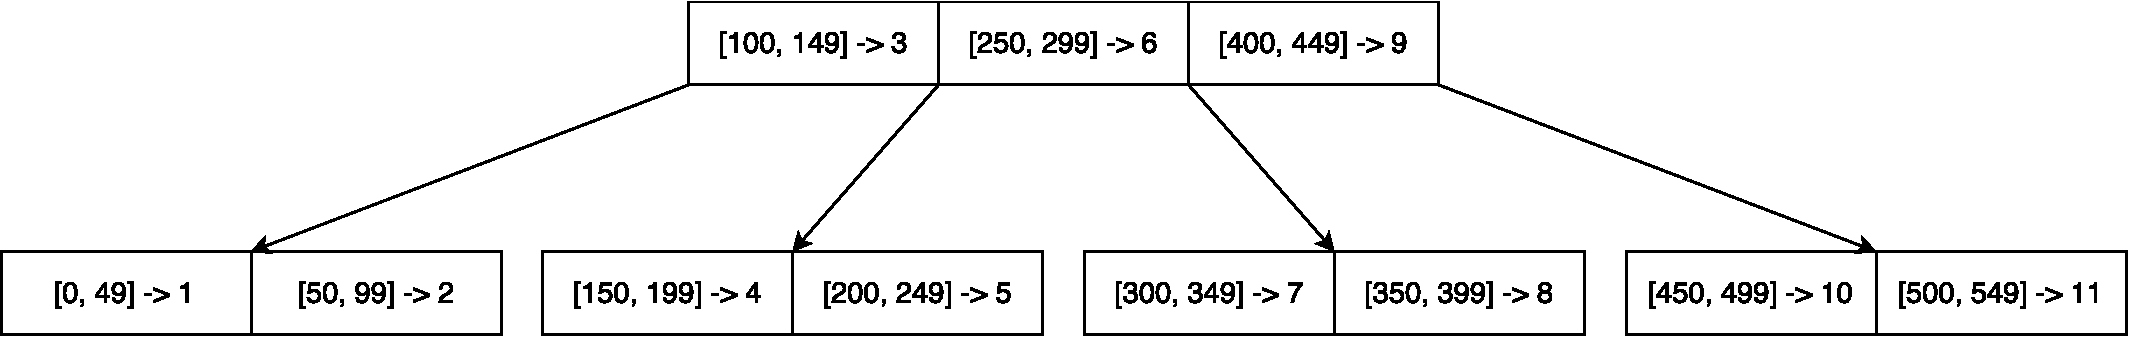
\includegraphics[width=\columnwidth]{figtree1.pdf}
        \caption{A FIG Tree constructed by creating an empty file and then extending it with 11 writes of 50 bytes each.}
        \label{fig:initfigtree}
    \end{subfigure}
    ~ %add desired spacing between images, e. g. ~, \quad, \qquad, \hfill etc. 
      %(or a blank line to force the subfigure onto a new line)
    \begin{subfigure}[b]{0.46\textwidth}
        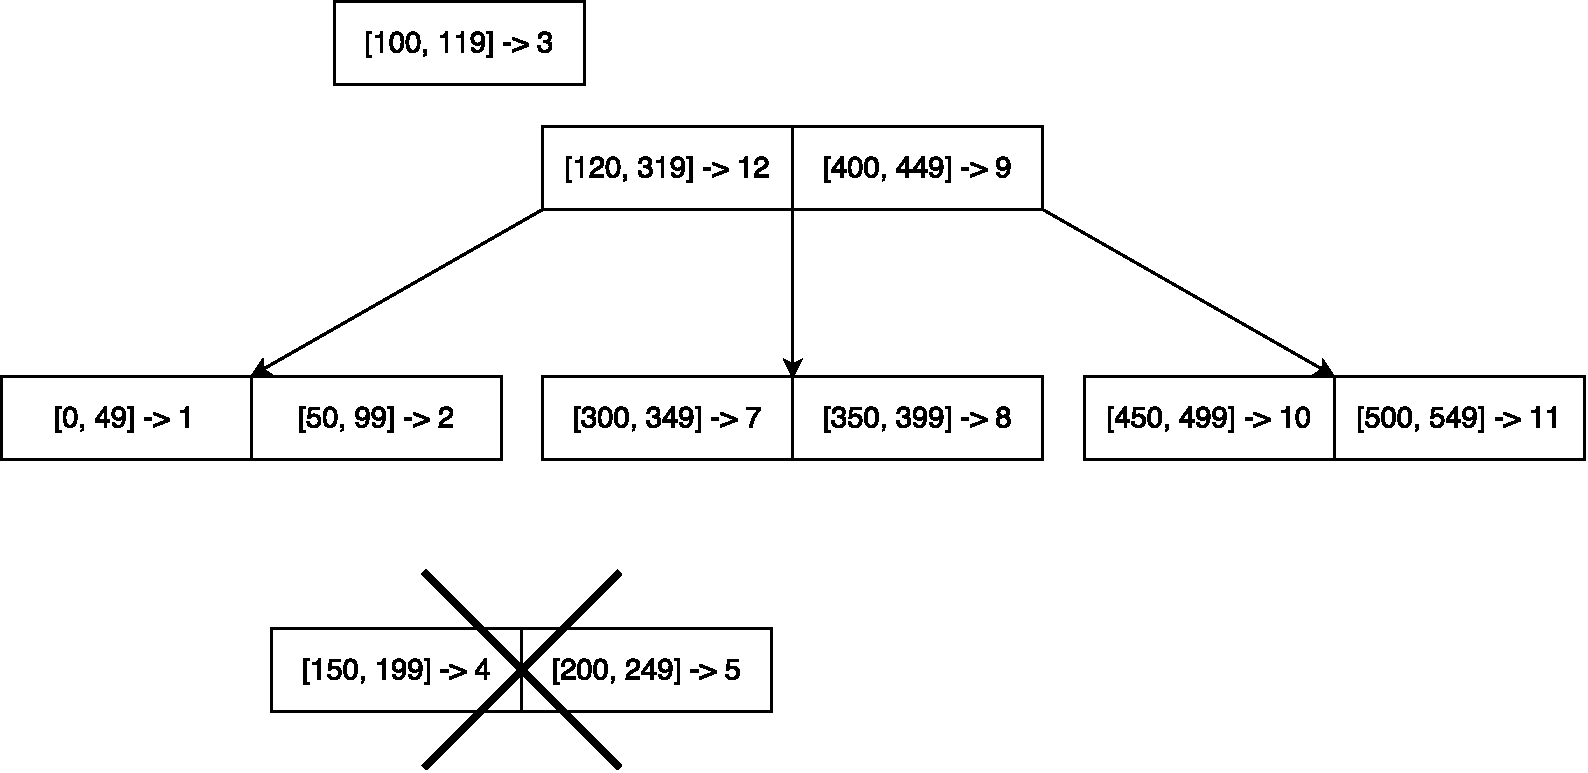
\includegraphics[width=\columnwidth]{figtree2.pdf}
        \caption{When a write of bytes 120 to 319 (inclusive) is performed, it replaces all entries in the root node that it overlaps with. The leftmost entry only partially overlaps with the range, so bytes 100 to 119 form a \emph{left continuation} that is inserted separately into the tree.}
        \label{fig:partialwritefigtree}
    \end{subfigure}
    ~ %add desired spacing between images, e. g. ~, \quad, \qquad, \hfill etc. 
    %(or a blank line to force the subfigure onto a new line)
    \begin{subfigure}[b]{0.52\textwidth}
        \begin{subfigure}[b]{\textwidth}
            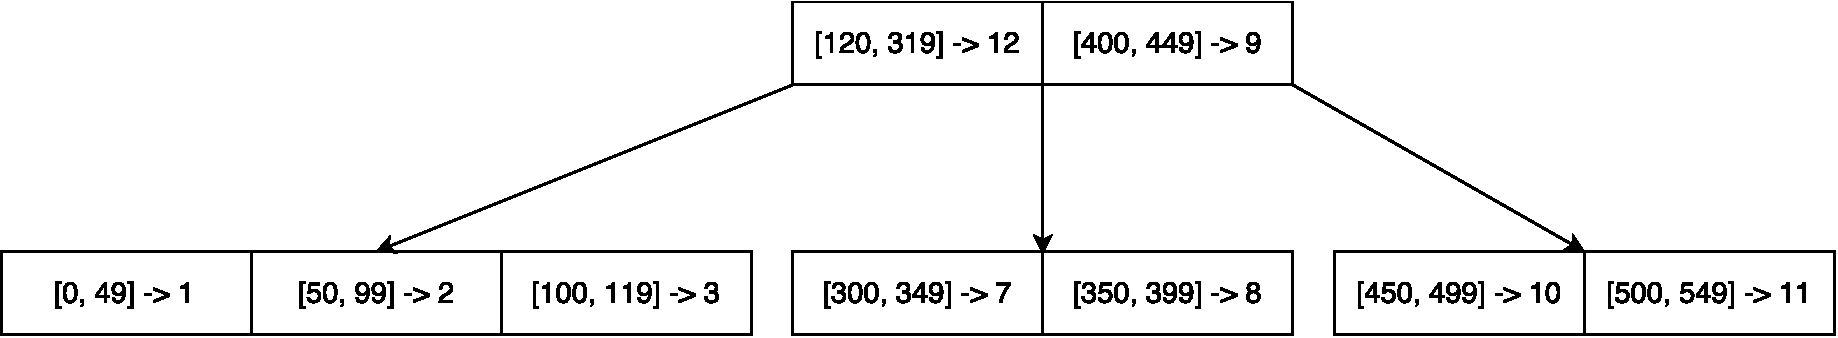
\includegraphics[width=\columnwidth]{figtree3.pdf}
            \caption{The final FIG tree, after bytes 120 to 319 are written.}
            \label{fig:afterwritefigtree}
        \end{subfigure}
        \begin{subfigure}[b]{\textwidth}
            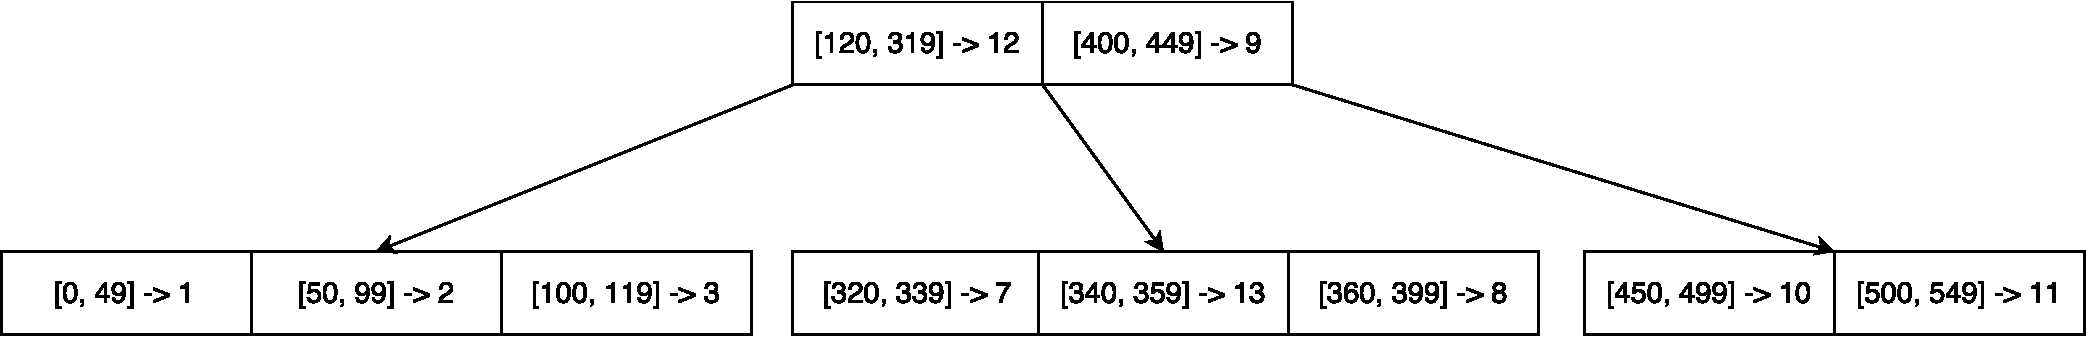
\includegraphics[width=\columnwidth]{figtree4.pdf}
            \caption{The final FIG tree after the additional write of bytes 340 to 369. Observe that the leaf node is pruned to the valid interval when it is written.}
            \label{fig:additionalwritefigtree}
        \end{subfigure}
    \end{subfigure}
    \caption{Example insertions into a FIG Tree.}\label{fig:figtree}
\end{figure*}

\subsection{Additional Optimizations}
Besides materializing files on the local disk and checkpointing files with FIG tree indices, we perform additional optimizations to improve performance of the GDPFS.

\subsubsection{Precreation of Logs}
One performance aspect that we quickly noticed when working on the filesystem is that file creation has high overhead. This stems from the fact that reads from a file are generally fast due to caching, and that writes to the GDP can be done asynchronously; in contrast, log creation must be done synchronously and is a bottleneck for workloads that create many files. Furthermore, logs cannot be created concurrently in the current version of the GDP, exacerbating this problem.

To alleviate this issue, we precreate logs ahead of time and add them to a queue, so that files can be created without having to wait for a synchronous remote procedure call to the log server to return. We implemented this as a synchronized bounded buffer, with a worker thread spawned on initialization of the filesystem that creates new logs and adds them to the bounded buffer whenever it is not empty. Threads that create files remove an element from the bounded buffer, or wait for the worker thread in case it is empty.

\subsubsection{Second-Chance List for Files}
One artifact of our file system is that opening a file for the first time is an expensive operation that requires multiple reads from the log server. In particular, it requires a synchronous read of the most recent log entry, which becomes a bottleneck when all reads are satisfied by the cache and all writes are done asynchronously. Therefore, we would like to mitigate this delay where possible.

One pattern that, on the surface, seems reasonable, is to checkpoint a file and deallocate the in-memory state of a file when all processes have closed it (it reaches a reference count of zero). However, we found that during compilation jobs, it is common for a file to be opened and closed many times. It is inefficient to deallocate a file when it is closed, only to perform a synchronous remote procedure call to rebuild that state when it is opened again.

Our solution to this problem was inspired by the demand paging algorithm used by the VAX operating system. Because the VAX operating system did not have hardware support for detecting when pages are used, it maintained ``hot" pages in memory in a FIFO list and a second-chance list in memory as an LRU list of pages marked ``invalid" in the page table. Pages that reach the end of the FIFO list of ``hot" pages are given a second chance in the LRU list before they are paged out to disk; a page that is accessed very rapidly will periodically enter the second-chance list before the ``hot" pages are in a FIFO list, but will never be paged out to disk because it will be ``revived" from the second-chance list on the next access.

Similarly, rather than deallocating the in-memory file structure when its reference count hits zero (i.e., when it is closed by all threads that opened it), we place the file on a second-chance list and maintain its in-memory state. If the file is opened soon after it is closed, then we no longer have to make synchronous remote procedure calls to rebuild its state, as we can simply ``revive" it from the second-chance list. To eventually reclaim resources, we stipulate that the second-chance list has a maximum size, and deallocate the in-memory state of a file when it reaches the end of the second-chance list. While we were developing the filesystem, we found that this optimization gave us a 100\% speedup for compilation jobs.

\section{Performance Evaluation}

\begin{figure}[t]
  \begin{subfigure}[b]{0.2\textwidth}
    \centering
    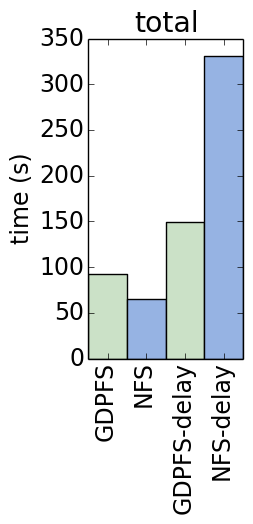
\includegraphics[width=.8\columnwidth]{total.png}
    \caption{Time to compile Redis in given filesystem. Results averaged over 3 trials.\label{fig:total}}
  \end{subfigure}
  ~
  \begin{subfigure}[b]{0.2\textwidth}
    \centering
    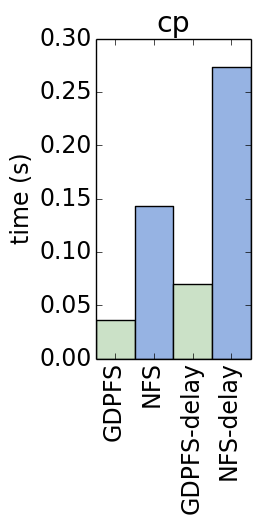
\includegraphics[width=.8\columnwidth]{cp.png}
    \caption{Time to cp zipped Redis tar into given filesystem. Results averaged over 3 trials.\label{fig:cp}}
  \end{subfigure}
  ~
  \begin{subfigure}[b]{0.2\textwidth}
    \centering
    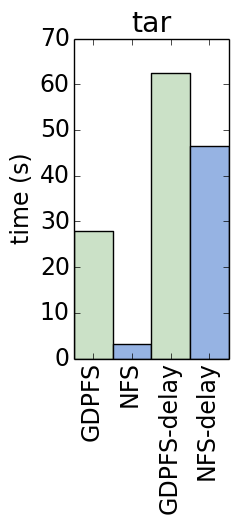
\includegraphics[width=.8\columnwidth]{tar.png}
    \caption{Time to unzip and untar Redis in given filesystem. Results averaged over 3 trials.\label{fig:tar}}
  \end{subfigure}
  ~
  \begin{subfigure}[b]{0.24\textwidth}
    \centering
    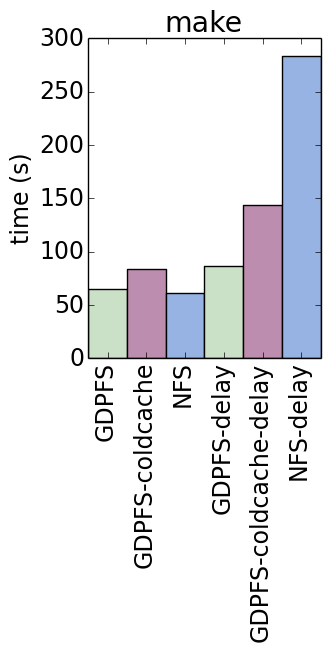
\includegraphics[width=.8\columnwidth]{make.png}
    \caption{Time to make Redis in given filesystem. Results averaged over 3 trials.\label{fig:make}}
  \end{subfigure}
  \caption{Macrobenchmark results.}
\end{figure}

Benchmark measurements were made on two hosts on the same LAN. The log server was run on a set of 2 Intel(R) Xeon(R) E5-2667 2.9GHz CPUs (6-Core, HT, 15MB Cache, 130W) with 64 GB (8 x 8GB DDR3-1600) of memory and 5 $\times$ 1 TB Seagate Constellation.2 (6Gb/s, 7.2K RPM, 64 MB Cache) 2.5" SATA drives in a RAID 6 configuration on a MegaRAID SAS 9260-16i controller. The remote client of the GDPFS was run on an Intel Core i7 processor, with 8 GB of memory and a 5400 RPM hard drive. The average latency between the two hosts is about 5 ms. In order to simulate running our file system in a Wide Area Network, we also ran experiments where we used the Linux's netem (Network Emulation) utility to artificially inject latency into our system. For these experiments, we added a latency of $10 \pm 2$ ms.

First, we discuss a macrobenchmark which tests our filesystem as a complete system and then we dive into microbenchmarks on file creation, sequential read, and sequential write performance. For each of our benchmarks, we compare against NFS a popular distributed filesystem. The NFS server is configured on the server with default settings and also mounted with default settings.

\subsection{Macrobenchmark: Redis}
The macrobenchmark we ran was to compile a popular key value store called \emph{Redis}. There are three steps to this benchmark: copying the tar file to the file system, untaring the archive, and finally making Redis. As a whole, we believe that these three steps accurately mimic a large proportion of use cases for our file system. 

\subsubsection{cp}

In Figure \ref{fig:cp}, we present the results for first copying the compressed tar into both the GDPFS and NFS. We found that in both the normal and the simulated WAN case, the GDPFS copied the tar in faster. We suspect that the cause is that the GDPFS returns from writes as soon as they hit the local filesystem, pushing them to the GDP asynchronously, whereas NFS may have to do some network I/Os to maintain cache coherency. That said, this is not a fair comparison because NFS supports more general semantics than the single-writer GDPFS. Because we assume a single writer, it is easier for the GDPFS to maintain cache coherence.

\subsubsection{tar}
NFS significantly outperformed the GDPFS in the tar step. This is because untarring requires creating many small files and the GDPFS is particularly bad at file creation, primarily for two primary reasons. First, since the GDPFS maintain a global mapping of file handles to file structs, the GDPFS must lock this structure when opening files. Thus when a large number of files are created and opened, there is a great deal of contention around the lock. Second, a bug in the current GDP implementation prevents us from creating logs concurrently so we are forced into synchronous creation of logs and we need one for each new file. We attempted to solve this problem by precreating a bounded buffer of logs, but we found that due to lock contention on the buffer we weren't using up the precreated logs. For further discussion, see Section \ref{sec:microbenchmark}.

\subsubsection{make}
Redis make times are comparable on NFS and the GDPFS in the simple case. However, in the simulated WAN case, we found that the GDPFS is significantly better than NFS. This led us to suspect that NFS was making more network round trips than the GDPFS, possibly to maintain a consistent cache.

We also tested make times for the GDPFS with a cold local cache. In this benchmark, the files were copied and untarred as normal, but then the GDPFS had its cache cleared before making. In all the other tests, reads and writes could be satisfied by the local cache. This benchmark was run in order to test the effectiveness of the FIG tree. The results demonstrate that the FIG tree keep the times for make at an acceptable level even with a cold cache. For more detailed results, see Figure \ref{fig:make}. 

\subsubsection{Total Times}
In total, we found that the time it takes to run all three stages (cp, tar, and make) on the NFS is slightly faster than on the GDPFS. However, when we added network latency into the benchmark we found that the GDPFS was significantly faster. This is due to the stricter single writer semantics of the GDPFS.

In summary, this macrobenchmark concludes that it is plausible to build a performant file system on top of append-only logs if enough caching and indexing layers are put in.

\subsection{Microbenchmarks}\label{sec:microbenchmark}
In order to get a more fine-grained view of the performance of the GDPFS we also ran three tests each of which stressed a main feature of file systems. These are: file creation, sequential writes, and sequential reads. These three tests were done in the same client and server as the macrobenchmarks. In addition, each of the tests also measures the performance in face of additional simulated latency.

\subsubsection{Creation Test}
In the creation test, we created a sequence of 3000 files and timed each call to the ``open" function, which we used to create files. We found that in both the normal and the delayed case, the NFS was faster at creating files. Because we are sequentially creating files in this microbenchmark, the earlier discussion about the file table lock is not applicable. 

We originally hypothesized that the explanation for this result was that we were running through the logs from our buffer of precreated logs. However, when we measured the size of our buffer we found that this was not the case. In fact, in all cases the buffer was either full or one away from being full. We suspect that this is because of lock contention on the bounded buffer. In the presence of multiple threads creating files (for example, in a compilation job), precreation of logs would likely improve performance.

\subsubsection{Write Test}
On each iteration of the write microbenchmark, we opened a file, appended 128 KiB of data, and closed the file. This process was repeated sequentially 100 times. We opened and closed the file on each iteration was to ensure that the filesystems were persisting the data and not just storing updates in an in-memory buffer. The reason we chose this chunk size is that FUSE prefetches reads in chunks of this size, and we wanted to make sure that the prefetching did not cause irregularities in our results.

Our results for this microbenchmark, which can be seen in figure \ref{fig:write}, reflect those seen in the cp macrobenchmark displayed in Figure \ref{fig:cp}. As stated in the section on cp, we believe this phenomena to be a result of the GDPFS returning from writes as soon as they hit the cache and then persisting them to the GDP asynchronously. In contrast, NFS must hit the network cache consistency before returning from a write.

\begin{figure}[t]
\centering
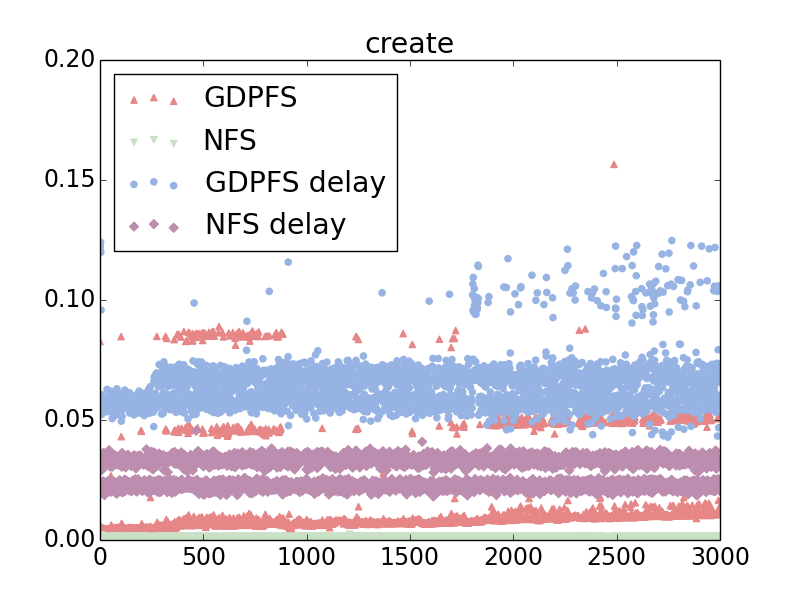
\includegraphics[width=.8\columnwidth]{create}
\caption{Distribution of times to create a file over 3000 files.\label{fig:create}}
\end{figure} 

\begin{figure}[t]
\centering
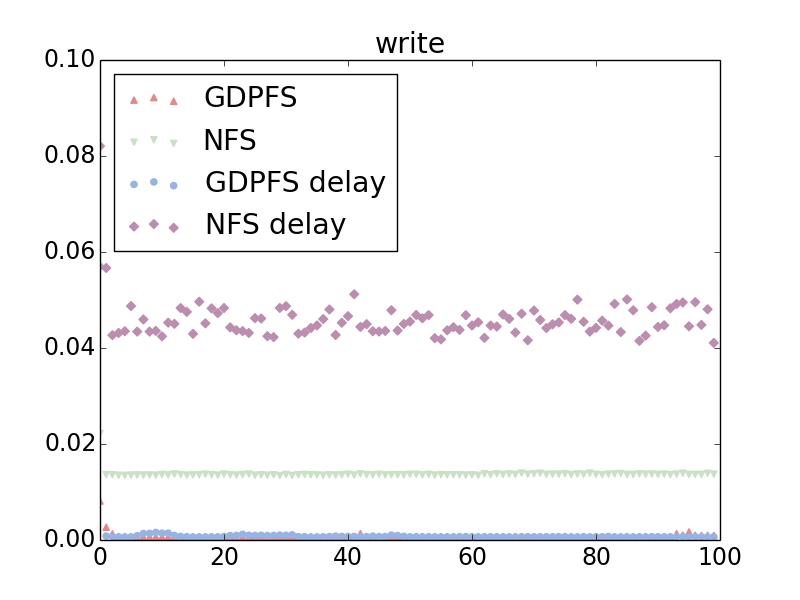
\includegraphics[width=.8\columnwidth]{write-open-close}
\caption{Distribution of times to write 32 blocks (128 KiB) over 100 writes.\label{fig:write}}
\end{figure} 

\begin{figure}[t]
\centering
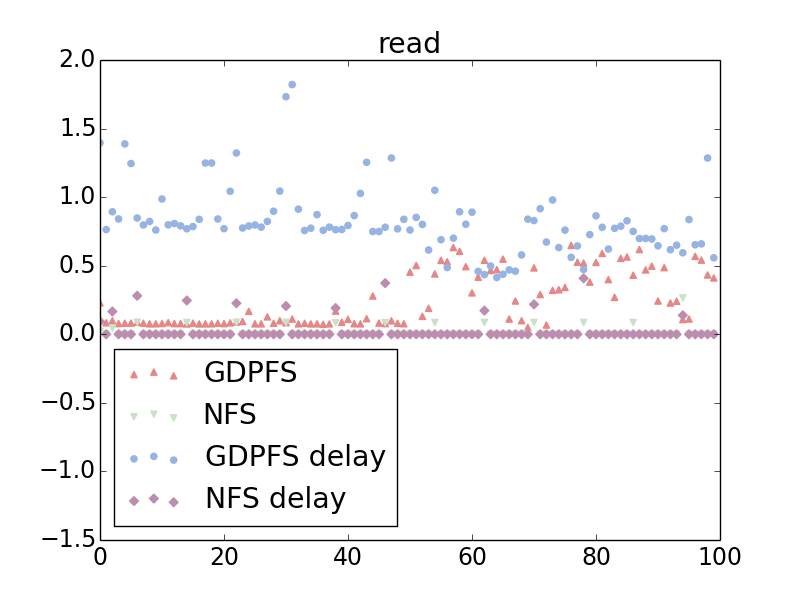
\includegraphics[width=.8\columnwidth]{read}
\caption{Distribution of times to read 32 blocks (128 KiB) over 100 reads.\label{fig:read}}
\end{figure} 

\subsubsection{Read Test}
In the read test, we unmounted and then remounted the filesystem in which we ran the write test. We then sequentially read the same 100 blocks from the file we wrote in the previous microbenchmark ensuring that each read still had the same data which was written.

In both cases, where we added network delay case and where we did not, the NFS significantly outperformed our GDPFS. There are two reasons for this. First, it seems that the NFS may have cached all of the data for the file upon opening it whereas the time to access the file is spread out across each read in the GDPFS. Second, because the NFS is working on top of a mutable backing store it is much easier for it to fetch the appropriate bytes. In the case of the GDPFS, since we had unmounted the file system earlier, each read had to be satisfied by a tree traversal and GDP synchronous read.

\section{Related Work}
Log based filesystems have been built before, most notably the Log-Structured Filesystem (LFS) \cite{LFS}. That said, we differ from LFS in a number of key areas. First, we are motivated to use logs because the GDP gives them to us with network access, distributed durability, atomicity and does this all with strong security guarantees over untrusted hardware. LFS uses logs because they allow writes without seeks. Second, every file in the GDPFS exists in its own log. Third, we do absolutely no modification in place. Everything is built around append only logs. LFS uses modify-in-place semantics in several areas including the checkpoint region. Fourth, we do away with traditional inodes and store file metadata in the log entries for each file. This means that a file in our system has no tie to the filesystem that it exists in and thus could theoretically be linked to in any other GDPFS mount. It also means that each file in the filesystem could potentially be owned by a different user\footnote{We did not implement this functionality and thus will leave it to future work.}.

Looking at file systems in general, the Network File System (NFS) \cite{NFS} and the Andrew File System (AFS) \cite{AFS}, being distributed file systems, bear great resemblance to the GDPFS. One of the most interesting contributions of AFS is its relatively weak semantics for concurrent modification of the same file. files are written back to the AFS server when they are closed, and the last close wins. These weak semantics are motivated by the observation that it is unlikely for multiple users to concurrently modify the same file. This same idea partially justifies the \emph{single-writer} nature of files in the GDPFS.

Because files are backed by logs, it is possible to ``go back in time" and restore an older version of a file. Our decision to use a separate log for each file allows files to be separately reverted to older versions. Some filesystems, such as the B-Tree Filesystem \cite{BTRFS}, use a Copy-on-Write strategy to cheaply snapshot files. However, the semantics of these snapshots are weaker than the versioning semantics achieved with a log.

There are a few other similar filesystems such as TahoeFS \cite{Tahoe} and the Fast Secure Filesystem (FSFS) \cite{FSFS}. However, they lack the copy on write and versioning advantages that our system provides. The GDPFS is novel because it is built solely on append-only logs, it gives strong atomicity guarantees, and can guarantee strong data integrity and confidentiality while running on a network at global scale and consisting solely of untrusted hardware.

\section{Future Work \& Lessons Learned}
Our goals in creating the GDPFS were (1) to make the GDP accessible to more applications, and (2) to evaluate the GDP as a useful primitive to create distributed systems.

We believe that we were fairly successful in achieving the first goal. Given that we only had limited time, we were unable to create a bug-free filesystem that was fully featured (with things such as hard links, symbolic links, etc.); however, we have made significant progress towards this end---we have created a filesystem that is stable enough to run compilation jobs of nontrivial systems. We believe that a few more months of development could turn the GDPFS into a usable file system. Many of the bugs hampering the stability of our file system are in the GDP itself, so much so that we feel that efforts should be taken to first make the GDP stable, before attempting to make our filesystem built on top of the GDP stable.

The second goal was to evaluate the usefulness of the GDP itself. First of all, it must not be forgotten that the GDP is itself a research project under active development. Furthermore, as far as we know our use case has put more stress on the GDP than anything anyone has previously done. That is, compared to other GDP applications we create more logs more quickly, do more frequent and larger batches of asynchronous reads and writes, and open and close a greater number of logs at a greater rate. Given this new stress, it is not a surprise that we found many new bugs. Much of our GDP-related friction was because of these bugs, so an obvious first step in improving the GDP's usefulness in building complex systems like ours is to fix these issues. That said, the fact that with a couple months of part time work we were able to construct a distributed filesystem that, with a few minor tweaks\footnote{We didn't quite implement all the security features in the GDPFS due to time constraints however the foundation is all there and we don't expect any performance changes since the GDPFS is by no means CPU bound.}, has the ability to securely operate over untrusted hardware, speaks to the advantages of using the GDP as a substrate for creating complex systems.

While the GDP enforces single writer semantics, there is no inherent reason why this restriction must be elevated to the level of the GDPFS. It would be interesting to figure out a way to restructure our system such that this limitation was removed. One could imagine a service, owned by a single entity (keypair), that was the ``single writer" of the filesystem, that provides the filesystem as a service to multiple logical writers. However, such a service would have to solve the cache coherency problems with multiple writers mentioned earlier. Furthermore, it would have to be replicated in order to be fault-tolerant, and, in order to scale at the level of the backing GDP, it would need to be able to run securely on untrusted hardware. In short, this system would have to implement much of the functionality provided by the GDP in such a way as to support multiple writers. Given that it would have to implement this functionality on its own anyway, we are unsure how it would benefit from using the GDP. The problem here is the \emph{single-writer} nature of GDP logs. While it provides convenient security properties, it is a shortcoming in that a multi-writer system needs to re-implement much of the functionality of the GDP to scale at that level.

The GDPFS could also be improved by implementing a system for accessing earlier versions of files. It would also be interesting to devise a key-sharing permission scheme to restrict which versions of a file are available to which readers.

\section{Conclusions}
In this paper, we have presented the GDPFS, which lifts the single-writer, append-only log abstraction provided by the Global Data Plane to a single-writer filesystem that is more usable for many applications. We have found that using the GDP enabled us to create a filesystem that---once the GDP is bug-free and production-ready---scales extremely well and runs on untrusted hardware. To our knowledge, no other distributed filesystem has been designed with these objectives in mind. However, we identified the single-writer nature of logs as a shortcoming of the GDP that prevents us from easily generalizing our filesystem to work in a multi-writer setting while still meeting the original objectives of extreme scaling and running on untrusted hardware.

\section{Acknowledgments}
We would like to thank the Global Data Plane Group within the Ubiquitous Swarm Lab at UC Berkeley for providing direction and support throughout the process of building the GDPFS. We would also like to thank Eric Allman specifically for aiding in the process of debugging and patching the GDP C client library and GDP log daemon when we ran into bugs that we could not work around.

%
% The following two commands are all you need in the
% initial runs of your .tex file to
% produce the bibliography for the citations in your paper.
\bibliographystyle{abbrv}
\bibliography{gdpfs-bib}  % bib.bib is the name of the Bibliography in this case
% You must have a proper ".bib" file
%  and remember to run:
% latex bibtex latex latex
% to resolve all references
%
% ACM needs 'a single self-contained file'!
%
\balancecolumns
% That's all folks!
\end{document}
